\chapter{\label{ch8-onsky}On-Sky Observations} 

\minitoc

\notes[inline,caption={}]{
	\section{Plan}
	\subsection{Topics}
	\begin{itemize}
		\item Decided upon reduction methods
		\item Potentially different than for performance chapter
		\item CHEC-M campaign
		\item MC CHEC-S
		\item Future observations
		\item Jupiter observations (Beyond cherenkov?)
	\end{itemize}
	\subsection{Questions}
	\begin{itemize}
		\item ?
	\end{itemize}
}

\section{Introduction}

\begin{figure}
  \begin{subfigure}[b]{0.49\textwidth}
    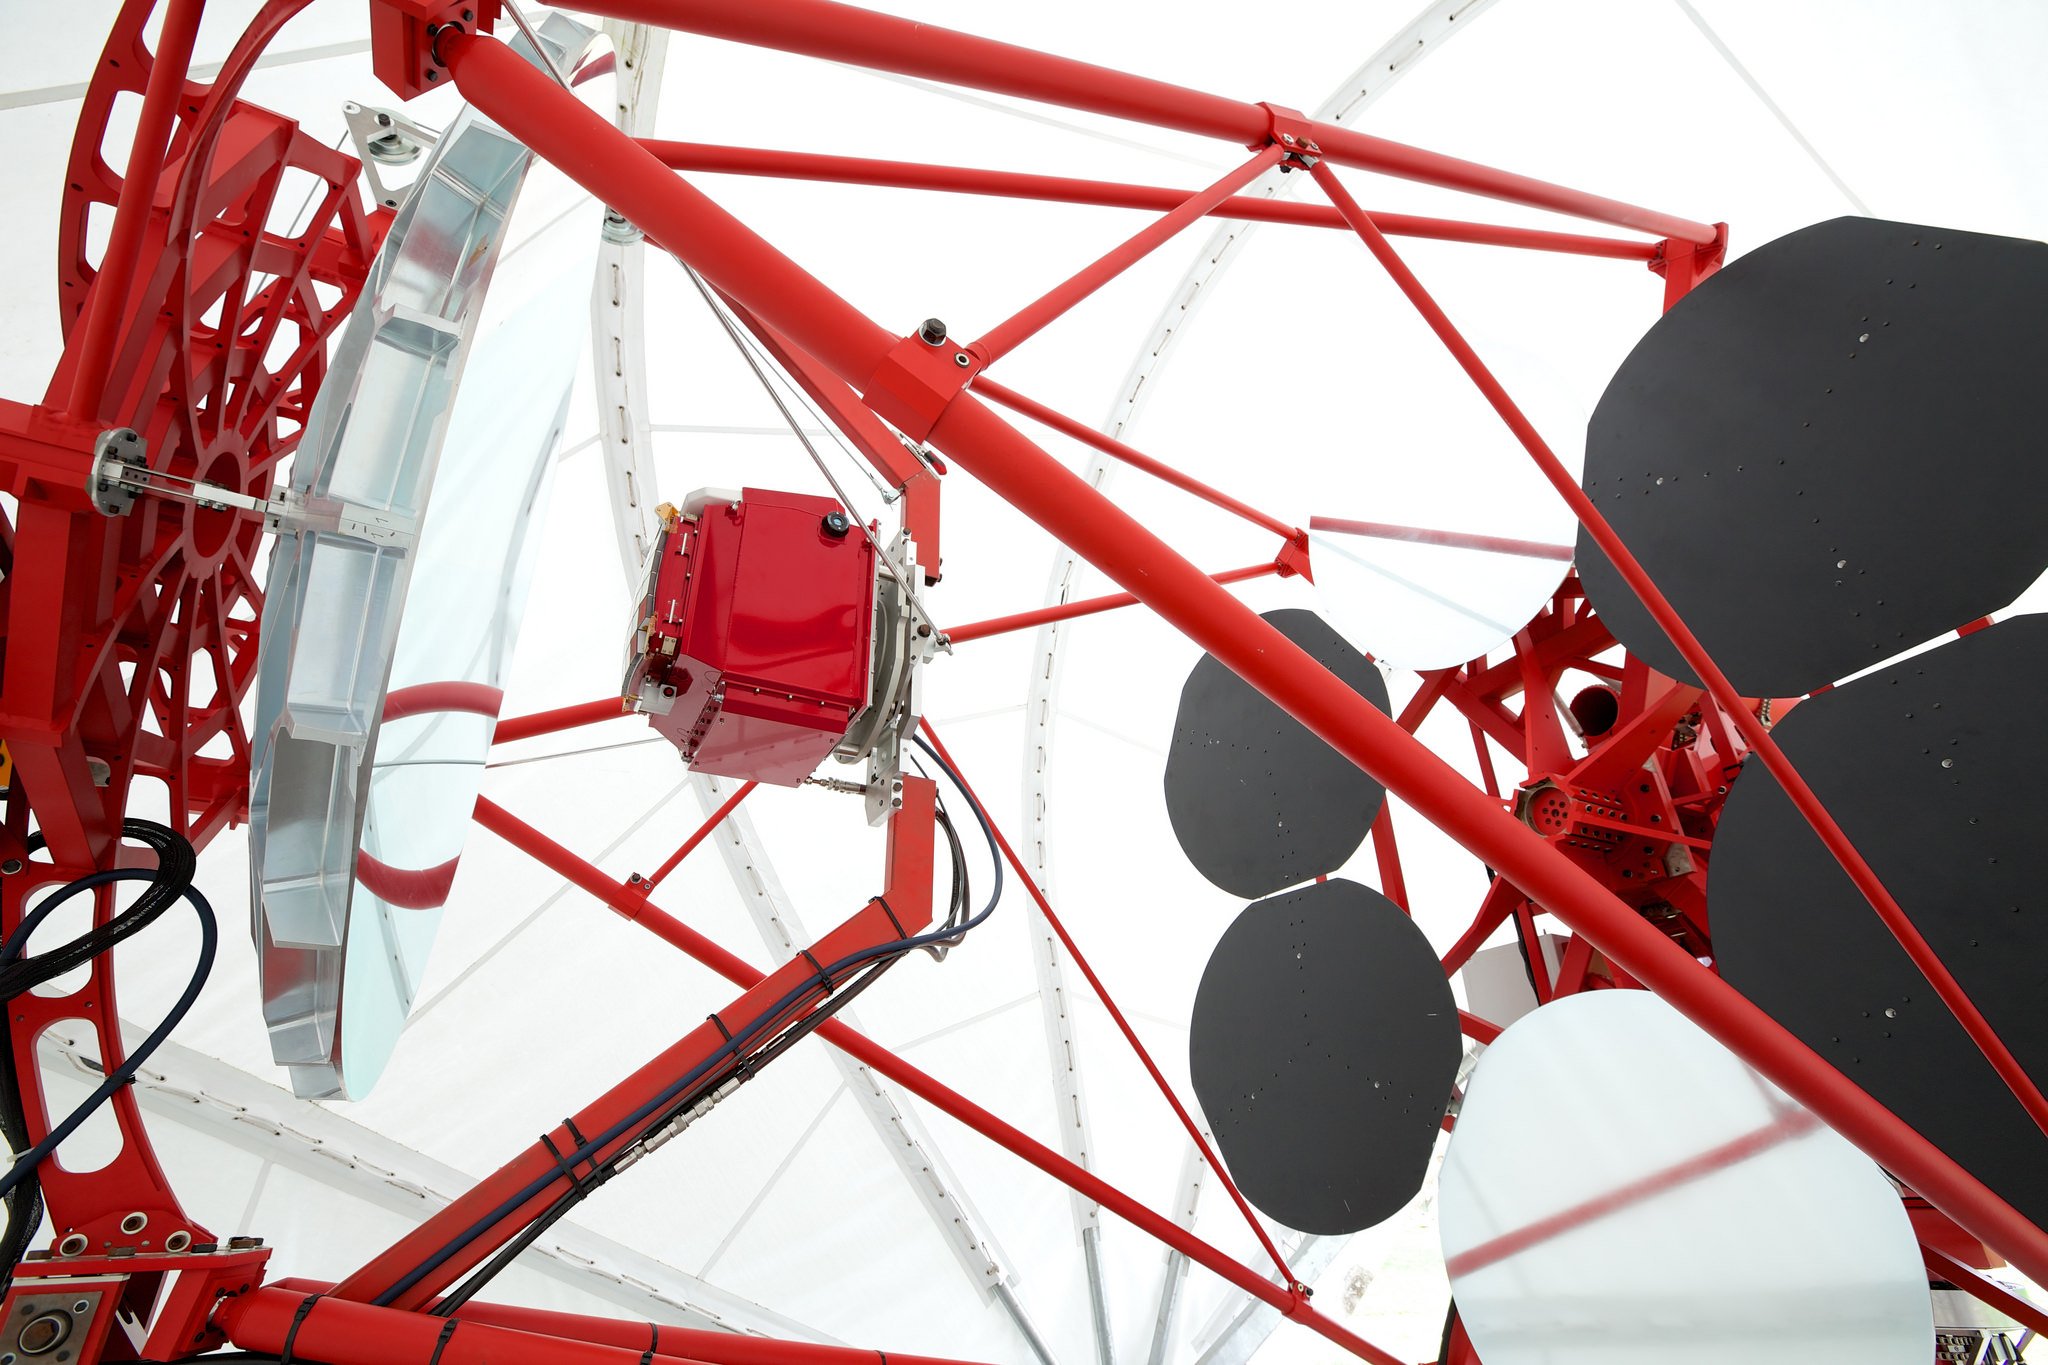
\includegraphics[width=\textwidth]{akira-telescope}
    \caption{Raw image.}
    \label{fig:r0_cherenkov_image_mirrored_cropped}
  \end{subfigure}
  \hfill
  \begin{subfigure}[b]{0.49\textwidth}
    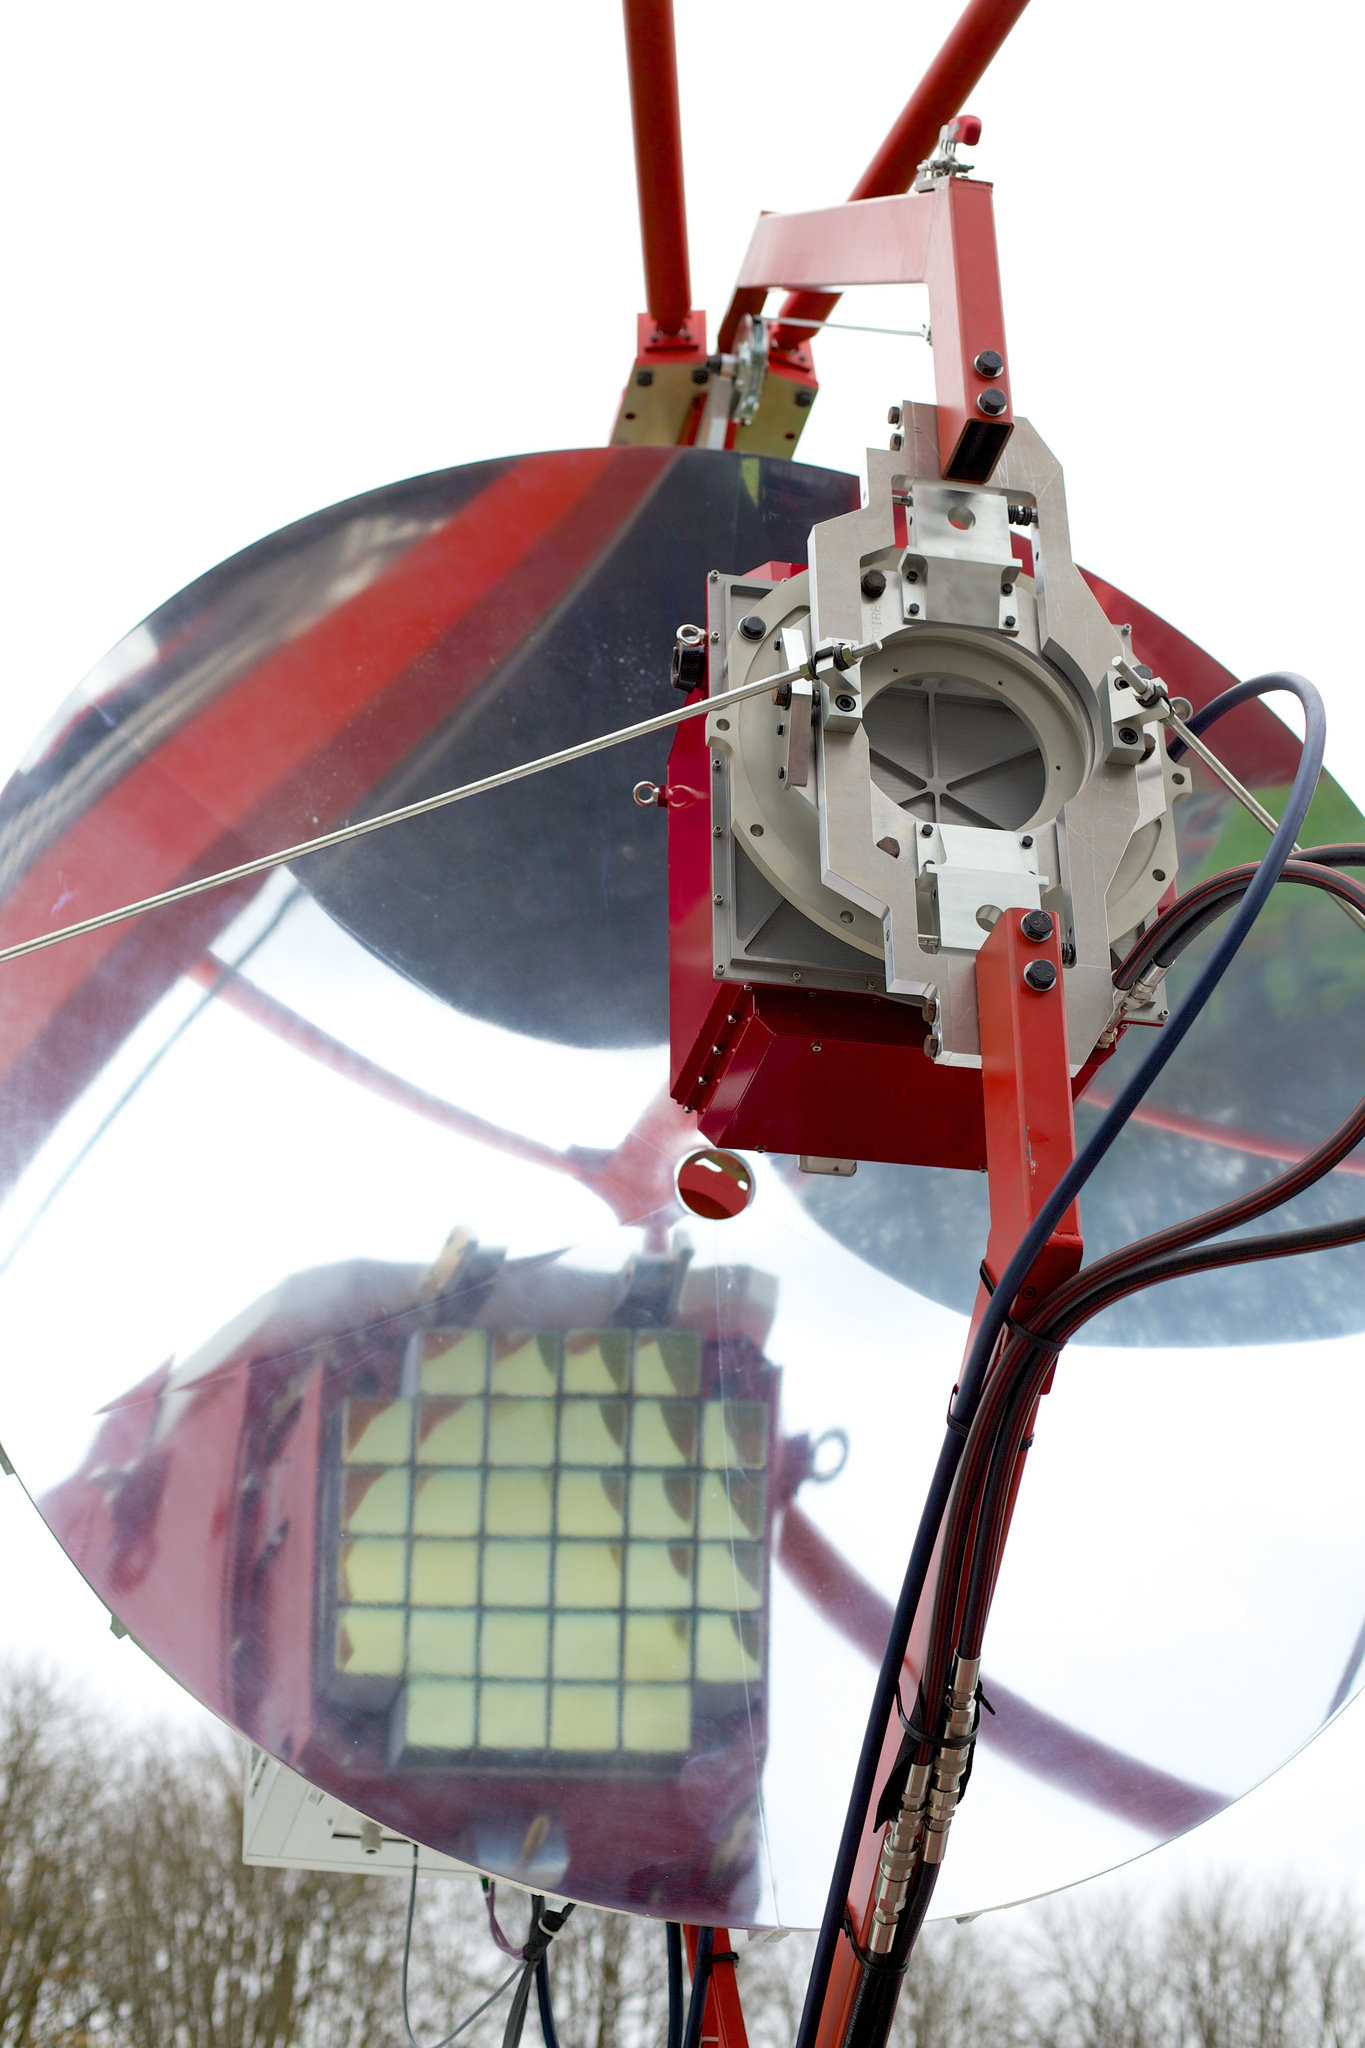
\includegraphics[width=\textwidth]{akira-reflection}
    \caption{Pedestal-subtracted image.}
    \label{fig:r1_cherenkov_image_mirrored_cropped}
  \end{subfigure}
  \caption[Comparison of calibration stages with a Cherenkov shower image.]{The same image of a Cherenkov shower taken with CHEC-M, but at different stages of calibration. An integration window was chosen using the \textit{Neighbour Peak Finding} technique (Chapter~\ref{ch6-reduction}) on the \si{\pe} calibrated waveforms. The same samples were then integrated for each of the calibration stages.}
\end{figure}

Testing the operation of the camera on the telescope structure is a very important part of the commissioning procedure. When on-telescope, the camera is in an environment we have very little control over, and is exposed to factors such as the \gls{nsb} from various sources, including moonlight, starlight, and artificial light pollution. The first on-telescope campaign took place during November 2015, at the location of the \gls{gct} telescope structure (Observatoire de Paris-Meudon), just before the inauguration of the \gls{gct} prototype. The primary intention of this campaign was to test the integration and operation procedure for \gls{chec-m} on the telescope structure, however the first detection of Cherenkov light from atmospheric showers by a \gls{cta} prototype camera was also achieved \cite{Watson2017}. 

After returning to the lab for further testing and characterisation, \gls{chec-m} was then re-installed on the \gls{gct} structure in March 2017 for a second on-telescope campaign. During this second campaign the \gls{gct} telescope was pointed towards two \gls{vhe} gamma-ray sources, Mrk421 and Mrk501. These two sources are blazar objects (\gls{agn} with a relativistic jet directed towards Earth) and were the first extragalactic \si{TeV} sources to be discovered \cite{Punch1992, Quinn1996}, testifying to their brightness. However, due to the high \gls{nsb} background that is present at the Meudon site (20 to 100 times brighter than expected at the final \gls{cta} site), the camera had to be operated at a low gain and high trigger threshold \cite{Zorn2017}. The combination of these operating conditions, and the limited observation time, meant an astrophysical detection was unlikely for this campaign. Nevertheless, Cherenkov showers were detected during the campaign. This chapter will describe the results I have obtained from the images of these Cherenkov showers.

\change{figure of camera on telescope, showing enclosure}

\section{Cherenkov Shower Images}

